% PLEASE USE THIS FILE AS A TEMPLATE
% Check file iosart2x.tex for more examples

% add. options: [seceqn,secthm,crcready,onecolumn]
\documentclass[sw]{iosart2x}
\usepackage{hyperref}
\usepackage{listings}

%\usepackage{dcolumn}
%\usepackage{endnotes}

%%%%%%%%%%% Put your definitions here


%%%%%%%%%%% End of definitions

\pubyear{0000}
\volume{0}
\firstpage{1}
\lastpage{1}

\begin{document}
\sloppy
\begin{frontmatter}

%\pretitle{}
\title{The Linked Connections framework for reliable historical and real-time data}
\runningtitle{The Linked Connections framework for reliable historical and real-time data}
%\subtitle{}

% For one author:
%\author{\inits{N.}\fnms{Name1} \snm{Surname1}\ead[label=e1]{first@somewhere.com}}
%\address{Department first, \orgname{University or Company name},
%Abbreviate US states, \cny{Country}\printead[presep={\\}]{e1}}
%\runningauthor{N. Surname1}

% Two or more authors:
\author[A]{\inits{D.}\fnms{David} \snm{Chaves-Fraga}\ead[label=e1]{dchaves@fi.upm.es}},
\author[B]{\inits{J.}\fnms{Julian} \snm{Rojas}\ead[label=e2]{julianandres.rojasmelendez@ugent.be}},
\author[B]{\inits{P.}\fnms{Pieter} \snm{Colpaert}\ead[label=e3]{pieter.colpaert@ugent.be}}
\author[A]{\inits{O.}\fnms{Oscar} \snm{Corcho}\ead[label=e4]{ocorcho@fi.upm.es}}
and
\author[B]{\inits{P.}\fnms{Ruben} \snm{Verborgh}\ead[label=e5]{ruben.verborgh@ugent.be}}
\runningauthor{Chaves-Fraga et al.}
\address[A]{Ontology Engineering Group, \orgname{Universidad Polit\'ecnica de Madrid}, \cny{Spain}}
\address[B]{IDLab, Department of Electronics and Information Systems, \orgname{Ghent University-imec}, \cny{Belgium}
\printead[presep={\\}]{e1,e2,e3,e4,e5}}

%\begin{review}{editor}
%\reviewer{\fnms{First} \snm{Editor}\address{\orgname{University or Company name}, \cny{Country}}}
%\reviewer{\fnms{Second} \snm{Editor}\address{\orgname{First University or Company name}, \cny{Country}
%    and \orgname{Second University or Company name}, \cny{Country}}}
%\end{review}
%\begin{review}{solicited}
%\reviewer{\fnms{First} \snm{Solicited reviewer}\address{\orgname{University or Company name}, \cny{Country}}}
%\reviewer{\snm{anonymous reviewer}}
%\end{review}
%\begin{review}{open}
%\reviewer{\fnms{First} \snm{Open Reviewer}\address{\orgname{University or Company name}, \cny{Country}}}
%\end{review}

\begin{abstract}
Using Linked Data based approaches a wide amount of companies and institutions share their data in an affordable way while allowing third parties to perform standard and federated queries. In transport domain, where a complex environment emerges, static, real-time and historical data have to coexist to provide reliable data to the information systems. Currently, however, public transport data is published in a way in which the processing is too expensive. In previous work, the Linked Connections (LC) framework was introduced as a cost-efficient publishing alternative to the \textit{de-facto} standard GTFS and route planning APIs. LC provides a light HTTP interface that allows smart clients to create their own route planners. We notice that at the moment in which historical and real-time are taken into account in the LC framework, some improvements are needed. Specifically in the case of live updates about the schedules, where it is important to maintain stable identifiers that remain valid over time.

This paper continues the previous work we have made for developing an affordable framework to publish reliable real-time and historical transport data. Our main contributions are: (i) a Linked Connections Real Time server that is able to process GTFS-RT feeds providing consistent identifiers, (ii) an efficient management of historical data taking into account the size of each fragments exposed on the Web and (iii) an implementation of multiple route planning algorithms to test if our approach provides reliable access to real-time and historical data. We evaluate and compare the contributions with our previous approaches where the distribution of the fragments were based on other variables, like the time. We discover that taking into account the size of the fragments has a relevant impact in the performance of query evaluation, as originally expected. In future work we would like to identify the optimal size of the fragments automatically, taking into account multiple variables like the geographical location or the type of transport.
\end{abstract}

\begin{keyword}
\kwd{Linked Connections}
\kwd{Historical Data}
\kwd{Real time data}
\kwd{Reliable data}	
\end{keyword}

\end{frontmatter}

%%%%%%%%%%% The article body starts:

%\section{}\label{s1}

%\subsection{}\label{s1.1}
\section{Introduction}\label{introduction} %Oscar and David
In the current state of the Web of Data, a wide amount of that data are exposed following the principles of Linked Data\cite{bizer2009linked}. Giving unique identifiers to each resource, representing the data using a shared and common vocabulary of the domain or the possibility of dereferencing each URI are some of the relevant aspects that made Linked Data as one the most common approaches to organize and expose the data on the Web\cite{heath2011linked}. This features allow third parties to query the data in a standard way, using for example, the corresponding query language for RDF, SPARQL\cite{prud2006sparql}, and the possibility of doing federation across multiple datasets\cite{buil2013federating}. However, today, a lot of domains need to deal with real-time and historical data where is important to maintain stable identifiers that remain valid over time. Transport is one of these domain, where a complex environment with multiple types of data sources have to be managed to provide reliable data to information systems.

Since May 2017, one of the main motivations for developing solutions about multimodal and integrated travel information services is the publication of the new directive by the EU Commission about discoverability and access to public transport data across Europe. This document proposes the making of public transport data from providers available on national or common access points saved on databases, data warehouse or repositories. All the states will provide access to a unique common point following different static standards as Transmodel\footnote{\url{http://www.transmodel-cen.eu}}, Datex II\footnote{\url{http://www.datex2.eu}} or GTFS\footnote{\url{https://developers.google.com/transit/gtfs}} and real-time standards GTFS-RT\footnote{\url{https://developers.google.com/transit/gtfs-realtime/}} or SIRI\footnote{\url{http://www.transmodel-cen.eu/standards/siri/}}. So the domain requires solutions able to provide reliable data and to deal with the heterogeneity of access points and the data formats.

One of the main challenges when the Linked Data approaches deal with transport domain, where real-time and historical data has to be taken into account for providing consistent data to the information services, is how to ensure that the identifiers of each resource is stable and valid over the time. For example, if we define the connection entity as a departure-arrival pair, in previous works on Linked Connections\cite{colpaert2015intermodal}, the URI of each connection was defined getting information from an static GTFS datasets. At the moment that real-time is involved, that URIs are not consistents because the real-time information has to be taken into account. An example of the conceptualization of a connection is shown in the Figure \ref{fig:connection}. Other relevant challenge is how to manage the exposed historical data on the Web to allow an optimal query performance. One of the requirements of most relevant route planning algorithms is that the data have to be sorted by the time. In previous works of Linked Connections\cite{rojas2017providing}, we developed a server that paginates the list of connections in departure time intervals (10 minutes) and publishes these pages over HTTP. We have noticed that the clients were able to analyze the historical data but the performance was too low.

\begin{figure}[t]
	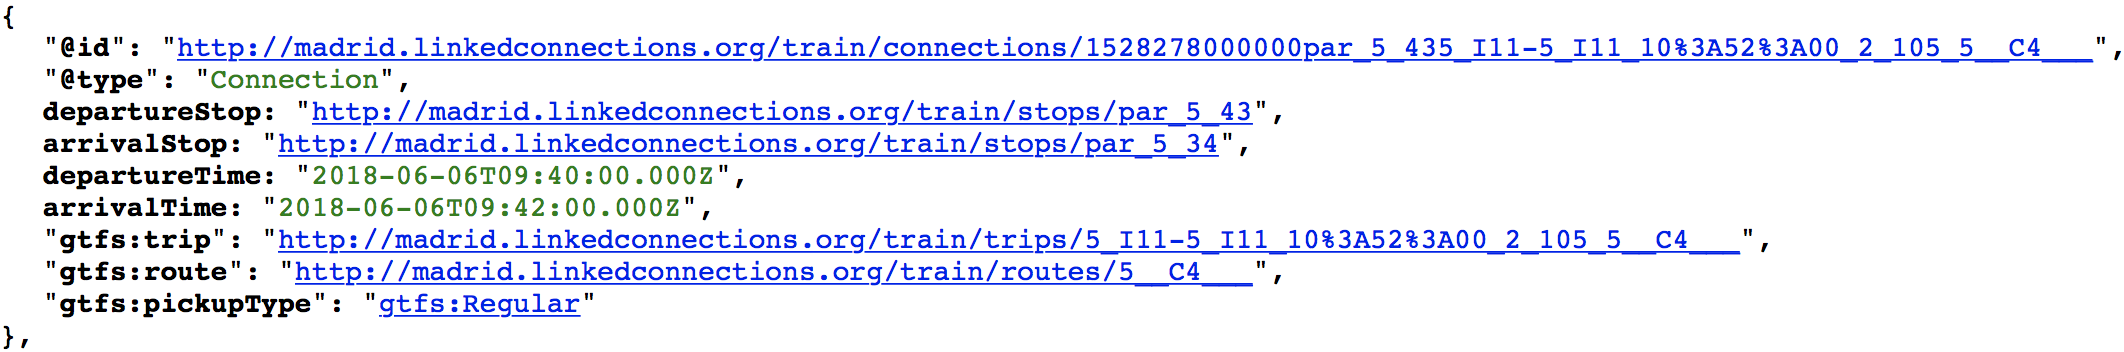
\includegraphics[width=0.47\textwidth]{images/connection.png}
	\caption{Example of a connection at LC in JSON-LD}\label{fig:connection}
\end{figure}

Our work is focused on providing an improvement of the current state of Linked Connections framework by allowing an efficient management of historical and real-time data with a standard vocabulary for the transport domain. This is relevant because two main reasons: (i) currently, a lot of transport companies are starting to provide access to their real-time services, but they the most common way to do it, is to develop an ad-hoc solutions like APIs or web services that only works locally \cite{colpaert2016public} and (ii) the heterogeneity of the domain in terms of data formats will be a very relevant problem next years, especially in Europe, based on the proposal of the EU Commission so a standard framework will be needed.  

In this paper we present the Linked Connections framework to provide reliable access to real-time and historical data. Our main contribution is the extension of previous version of the LC server, by providing an efficient management of real-time and historical data. First, we develop a library that gets information from static GTFS datasets and GTFS-RT data streams and exploit and integrate them following the LC vocabulary. Second, we modify the approach of Linked Connections for splitting the fragments of the data using a specific size of each fragment instead of the time. Third, we program a set of route planning algorithms in the top of the LC server to test if our approach is able to provide reliable data. Finally, we evaluate the improvements comparing the new version of the LC framework with our previous approaches, as base line.

The paper is organized as follows: Section 2 presents some of the related work about relevant approaches about exposing data on the web efficiently,  previous steps about the Linked Connections framework, a description of the \textit{de-facto} standard GTFS and the specification of relevant route planning algorithms. Section 3 describes our proposal about the improvements of the Linked Connections framework. Section 4 presents the design of our experiments. Section 5 describes the results we obtained evaluating our main contributions. Section 6 provides a brief discussion about the relevance of our contributions, and Section 7 presents conclusions and areas for future work.



\section{Related Work}\label{related_work} %David
On the current state of the Web, huge amount of data are exposed following the principles of Linked Data. In this section, we describe the main contributions on this topic focused on an efficient exposition and on the transport domain, a description of previous approaches developed using the Linked Connections framework and the analysis of the model for transport data, GTFS, that supports our work. Finally we analyse the most relevant algorithms for route planning.

One of the most well-known alternatives to publish data on the Web is Linked Data \cite{bizer2009linked}. Linked Data allows to identify in an unique way resources on the Web using identifiers, or HTTP URIs. It is a method to distribute and scale data over large organizations such as the Web. When looking up this identifier by using the HTTP protocol or using a Web browser, a definition must be returned, including links towards potential other interesting resources, a practice called \textit{dereferencing}. The triple format to be used in combination with URIs is standardized within RDF. The URIs used for these triples already existed in other data sources, and we thus favoured using the same identifiers. It is up to a data publisher to make a choice on which data sources can provide the identifiers for a certain type of entities. 

A common problem in Linked Data is the availability of the triple stores. They provide a way to getting data using the SPARQL query language but at the moment of queries involved long periods of time, these approaches are not efficient\cite{verborgh2014querying}. The Linked Data Fragments(LDF)\cite{verborgh2016triple,verborgh2014web} solve this issue fragmenting the data in several HTTP documents. Following this approach the store moves the load from server side to client side improving its availability. Comunica\cite{taelman2018comunica} is a framework that extends the possibilities of LDF, allowing to query other semantic interfaces as common SPARQL endpoint, RDF data dumps or HDT datasets\cite{fernandez2013binary}. 

Linked Connections\cite{colpaert2015intermodal} applies this approach to develop an cost-efficient solution based on a HTTP interface for transport data. The main assumption of LC  is that the relevant data for route planners can be based on the connection concept. Basically, as the LC vocabulary\footnote{\url{http://semweb.mmlab.be/ns/linkedconnections}} defines it, a connection describes a departure at a certain stop and an arrival at a different stop with their corresponding departure and arrival times and without any intermediate stop. A basic implementation of LC is shown in Figure \ref{fig:lc_imp}, where the route planning algorithms have to analyse the connections (small rectangles) through the pages (big rectangles) and across the time to find the expected route. The join between the connections is possible because same resources have same identifiers, based on one of the principles of Linked Data. The Hydra Ontology\cite{lanthaler2013hydra} is used to specify the next and previous page links as well as how the resource itself should be discovered


\begin{figure}[t]
	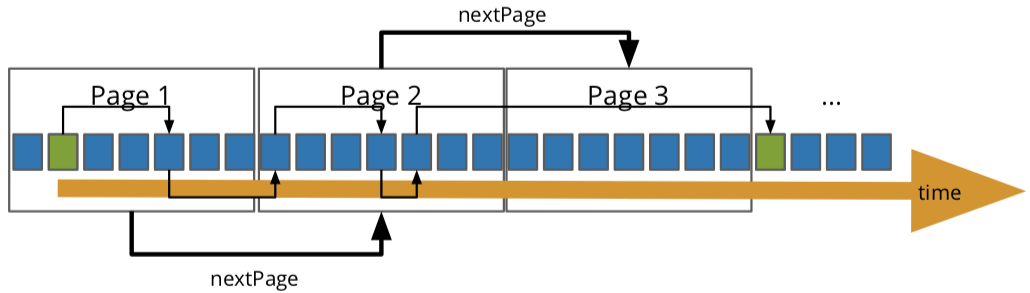
\includegraphics[width=0.47\textwidth]{images/implementation.png}
	\caption{Linked Connections implementation}\label{fig:lc_imp}
\end{figure}

It also relevant to describe the previous works that has been carried out using the specification of Linked Connections. For example, \cite{colpaert2017public} describes a analyse the behaviour of a basic transport API and the Linked Connections framework for public transit route planning, comparing the CPU and query execution time. The authors found that, at the expense of a higher bandwidth consumption, more queries can be answered using  LC than the origin-destination API. In \cite{colpaert2016impact} studies the impact of taking into account user preferences in a public transit route planning adding that features both on server and client and comparing the two solution on query execution time, cache performance and CPU usage on both sides. A first step for providing reliable access to historical and real-time data using Linked Connections is described in \cite{rojas2017providing}, where a mechanism is introduced to tackle the problem of the management of  data modifications when real-time is involved in route planning queries. Tripscore\footnote{\url{www.tripscore.eu}}, a Linked Data client that consume several Linked Connections servers with real-time and historical data is also described in \cite{ChavesFragaEtAl:DeSemWeb2017}, where the Connection Scan Algorithm (CSA) is implemented as the route planning algorithm in top of the client\cite{dibbelt2013intriguingly}. Tripscore add multiple user preferences at the client side to provide an score for each possible route. 

All the solutions that we aforementioned are rely on the \textit{de-facto} standard for representing public transport data, the General Transit Feed Specification or GTFS. This model, and its extension for real-time (GTFS-RT) is used by Google Maps\footnote{\url{http://maps.google.es}} since 2005 but also by other route planners like Open Trip Planner \footnote{\url{http://www.opentripplanner.org}} or  Navita.io\footnote{\url{https://www.navitia.io}}. It is also the most common model used by the transport companies to expose their data on open data portals, like for example the Consorcio General de Transportes de Madrid\footnote{\url{http://datos.crtm.es}}, the TRAM in Barcelona\footnote{\url{https://opendata.tram.cat/}} or the Belgium National Train System (SNCB). GTFS defines the headers of 13 types of CSV files and a set of rules the must be take into account when the dataset is created. Each file, as well as their headers, can be mandatory or optional and the have relations among them as show in Figure \ref{fig:gtfs}. Linked Connections is getting the necessary information from a subset of the full dataset:

\begin{itemize}
	\item stops: Individual locations where vehicles pick up or drop off passengers.
	\item calendar: Dates for service IDs using a weekly schedule. Specify when service starts and ends, as well as days of the week where service is available.
	\item calendar\_dates: Exceptions for the service IDs defined in the calendar file.
	\item stop\_times: Times that a vehicle arrives at and departs from individual stops for each trip.
	\item trips: Trips for each route. A trip is a sequence of two or more stops that occurs at specific time.
	\item routes: Transit routes. A route is a group of trips that are displayed to riders as a single service.
	\item transfers: Rules for making connections at transfer points between routes.
\end{itemize}

In order to link the terms and identifiers define in these files with the Linked Open Data cloud, we used the Linked GTFS\footnote{\url{http://vocab.gtfs.org/terms}} vocabulary. We create mappings able to transform GTFS files to Linked GTFS following the CSV2RDF\cite{tennison2015model} W3C recommendation\footnote{\url{https:// github.com/ OpenTransport/ gtfs- csv2rdf}} but also using other standard OBDA mapping languages that are able to deal with CSV files\footnote{\url{https://github.com/dachafra/gtfsmappings}}, like RML\cite{dimou2014rml} or R2RML\cite{das2012r2rml}. 

\begin{figure}[t]
	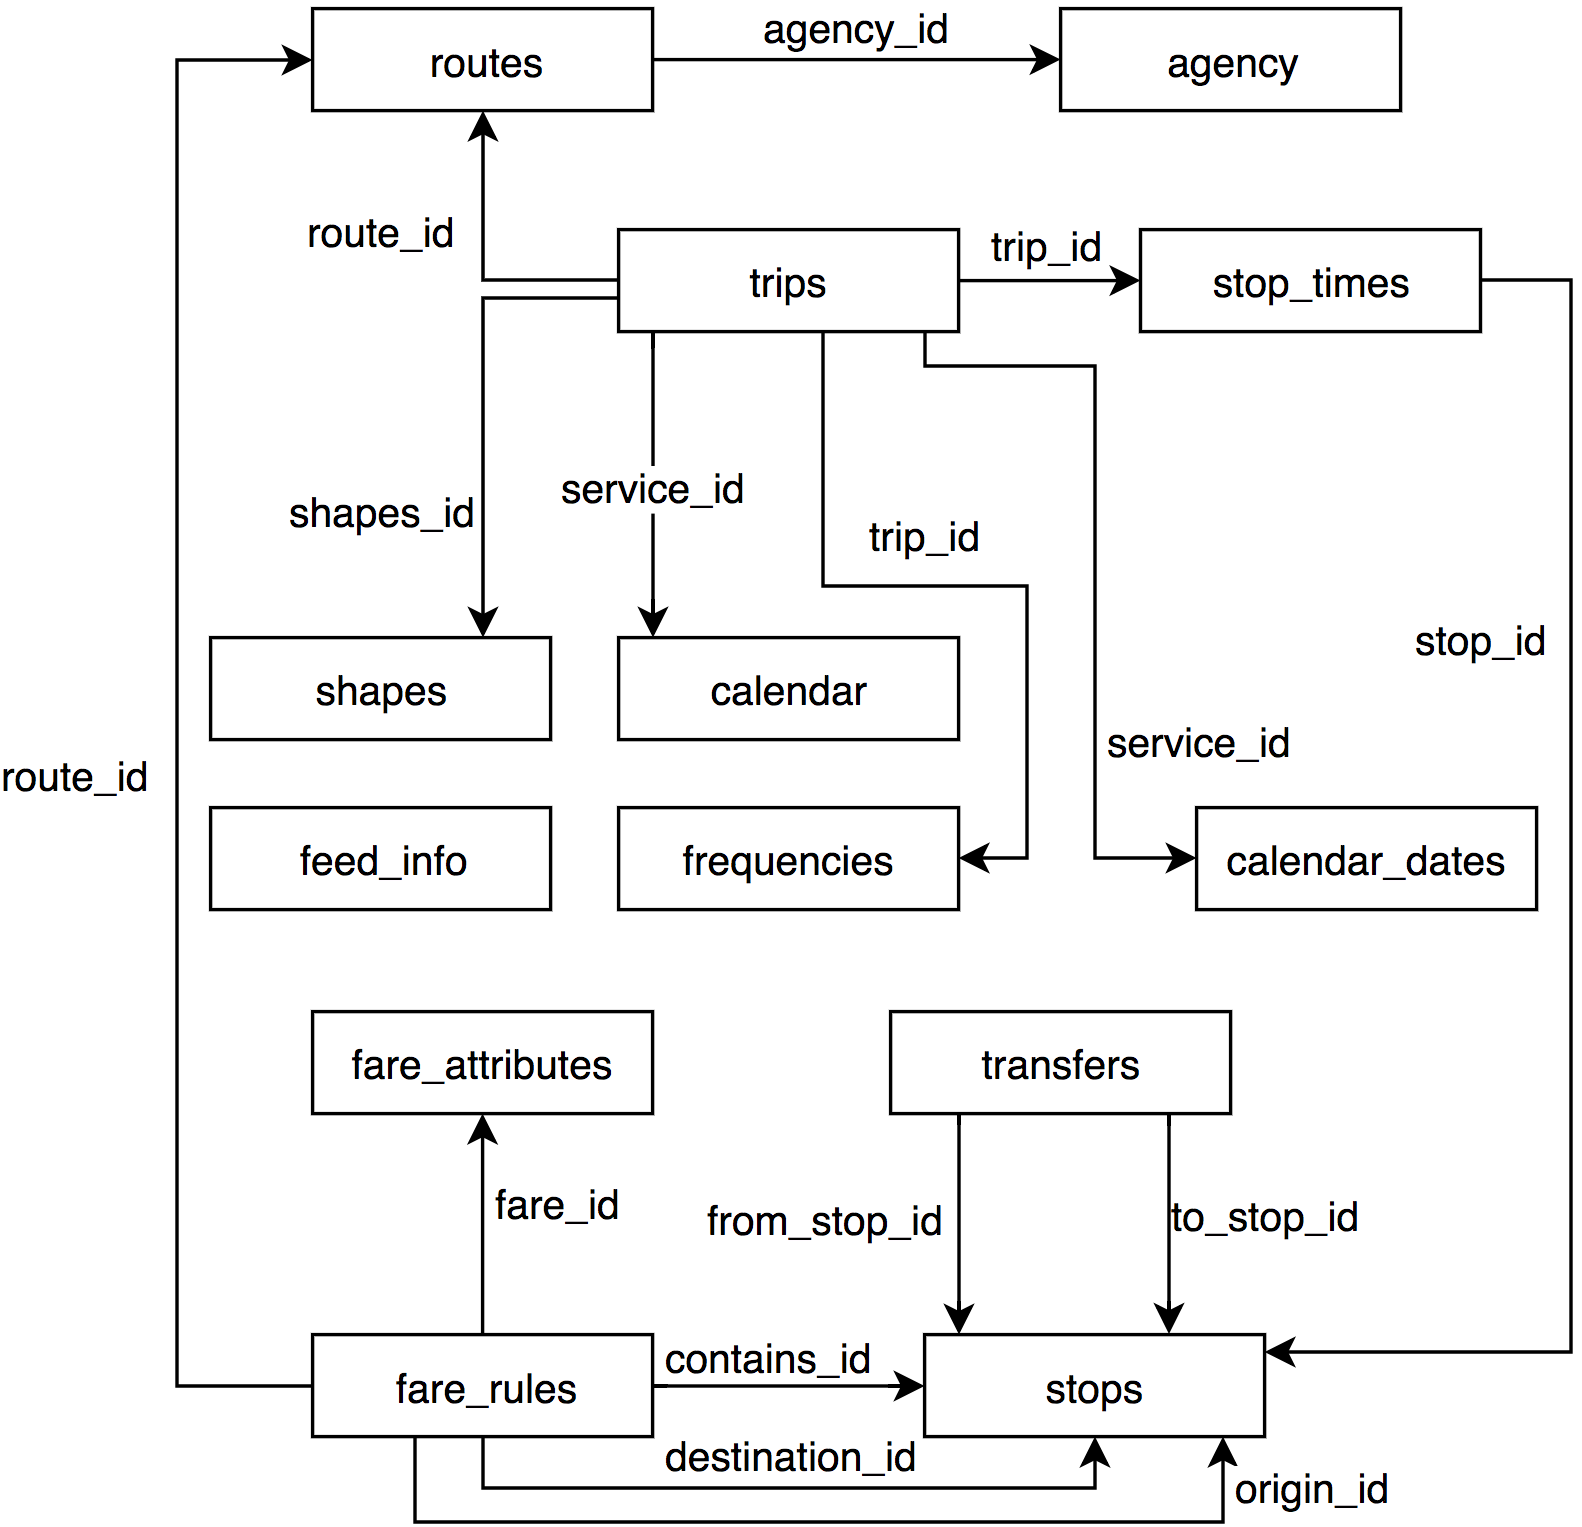
\includegraphics[width=0.47\textwidth]{images/gtfsmodel.png}
	\caption{The GTFS model and its primary relations}\label{fig:gtfs}
\end{figure}

The extension of GTFS for real-time, GTFS-RT\footnote{\url{https://developers.google.com/transit/gtfs-realtime/}} is a feed specification that allows public transport agencies to provide realtime updates about their fleet. The specification supports three types of information: (i) trips updates like delays, cancellations or change routes, (ii) service alerts like stop moved, unforeseen events affecting stations, routes, etc and (iii)  information of vehicle positions  including location and congestion level. The data exchange format is based on Protocol Buffers\footnote{\url{https://developers.google.com/protocol-buffers/}}.

It is also important to mention the works about route planning algorithms, that can be developed on the top of the Linked Connections framework. The problem that these algorithms has to solve using the data is the Earliest Arrival Time (EAT). An EAT query consists of a departure stop, a departure time and a destination stop. The main goal is to find the fastest journey to the destination stop starting from the departure stop at the departure time. There are more complex route planning questions like the Minimum Expected Arrival Time (MEAT)\cite{dibbelt2013intriguingly} or \textit{multi-criteria profile} queries\cite{bast2010fast,delling2014round,witt2015trip}. The Connection Scan Algorithm (CSA) \cite{dibbelt2013intriguingly} is an approach that models the timetable data as a directed acyclic graph \cite{strasser2014connection} using a stream of connections. As we defined before, a connection is a combination of a \textit{departure stop} ($c_{depstop}$) with a \textit{departure time} ($c_{deptime}$) and an \textit{arrival stop} ($c_{arrstop}$) with an \textit{arrival time} ($c_{arrtime}$). All the connections are combined in a stream of connections, sorted by increasing departure time. Thanks to this feature, it is sufficient to only consider the connections where the $c_{deptime}$ is later than the desirable departure time. The CSA algorithm works as follows, when a new scanned connection leads to a faster route to the arrival stop, the minimum spanning tree (MST) will be updated. This is the case when $c_{arrtime}$ is earlier than the actual EAT at $c_{arrstop}$, Finally the algorithm ends when the destination stop is added to the MST and the resulting journey can be obtained by following the path in the MST backwards.

In summary, after some proofs of concepts developed taking into account real-time and historical data in the LC framework and the current advances in the state of the work exposing the data on the Web efficiently, we think that it is the moment to improve the features of the current LC framework to create a standard mechanism for publish reliable public transport data. The main motivations to do that are, on one hand, the necessity to improve the current access of the transport information services to the data, where at the moment that real-time is involved, the solutions are basically ad-hoc and they are not feasible if we are based on the proposal of the EU Commission for publish public transport data. On the other hand, supported by the characteristics of the transport data, where a complex data management environment emerges, the new approach that we present in this paper can serve as a source of inspiration for historical and real-time Linked Data management on the Web in other domains.


%EU comission proposal?

\section{The Linked Connections Framework}
In this section, we describe the Linked Connections framework for providing reliable access to real-time and historical data. First, we describe a summary of the Linked Connections specification including new properties about features of real-time data. Second, we describe the extensions we develop to deal with these types of data: the linked connections library for transforming real-time feeds into connections and the LC server for managing and exposing that connections on the Web efficiently.

\subsection{The Linked Connections specification}

The LC specification\footnote{\url{https://linkedconnections.org/specification/}} explains the how to implement a data publishing sever, and explains what you can rely on when writing a route planning client. Following the Linked Data principles and the REST constraints, we make sure that from any HTTP response, hypermedia controls can be followed to discover the rest of the dataset. A "Linked Connections graph" is a paged collection of connections, describing the time transit vehicles leave and arrive. The Linked Connections vocabulary\footnote{\url{http://semweb.mmlab.be/ns/linkedconnections\#}} defines the basic properties to used with the \texttt{lc:Connection} class:
\begin{itemize}
	\item \texttt{lc:departureTime} It is a date-time, including delay, at which the vehicle will leave for the \texttt{lc:arrivalStop}.
	\item \texttt{lc:departureStop} The departure stop URI.
	\item \texttt{lc:departureDelay} Provides time in seconds when the \texttt{lc:departureTime} is not the planned departureTime.
	\item \texttt{lc:arrivalTime} It is a date-time, including delay, at which the vehicle will arrives at \texttt{lc:arrivalStop}.
	\item \texttt{lc:arrivalStop} The arrival stop URI.
	\item \texttt{lc:arrivalDelay} Provides time in second when the \texttt{lc:arrivalTime} is not the planned arrivalTime.
\end{itemize}

We also reuse the terms from the Linked GTFS vocabulary\footnote{\url{http://vocab.gtfs.org/terms}} in order to describe other properties of a \texttt{lc:Connection} class. This vocabulary it is aligned with the \textit{de-facto} standard to exchange public transport data on the Web, GTFS:

\begin{itemize}
\item \texttt{gtfs:trip} Must be set to link a a \texttt{gtfs:Trip} with a \texttt{lc:Connection}, identifying whether another connection is part of the current trip of a vehicle.
\item \texttt{gtfs:pickupType} Should be set to indicate whether people can be picked up at this stop. The possible values: \texttt{gtfs:Regular}, \texttt{gtfs:NotAvailable}, \texttt{gtfs:MustPhone} and \texttt{gtfs:MustCoordinateWithDriver}.
\item \texttt{gtfs:dropOffType} Should be set to indicate whether people can be dropped off at this stop. The possible values are the same as the defined in the \texttt{gtfs:pickupType} property.
\end{itemize}

It is important to remark that each Linked Connections page must contain some metadata about itself. The URL after redirection, or the one indicated by the Location HTTP header, therefore must occur in the triples of the response. The current page must contain the hypermedia controls to discover under what conditions the data can be legally reused, and must contain the hypermedia controls to understand how to navigate through the paged collection(s). A different ways exist to implement the paging strategy. At least one of the strategies must be implemented for a Linked Connections client to fin the next pages to precessed:
\begin{enumerate}
\item Each response must contain a \texttt{hydra:next} and \texttt{hydra:previous} page link.
\item Each response should contain a \texttt{hydra:search} describing that you can search for a specific time, and that the client will be redirected to a page containing information about that timestamp. To describe this functionality the \texttt{hydra:property} \texttt{lc:departureTimeQuery} is used. An example is shown in the Figure \ref{fig:metadata}
\end{enumerate}

\begin{figure}[t]
	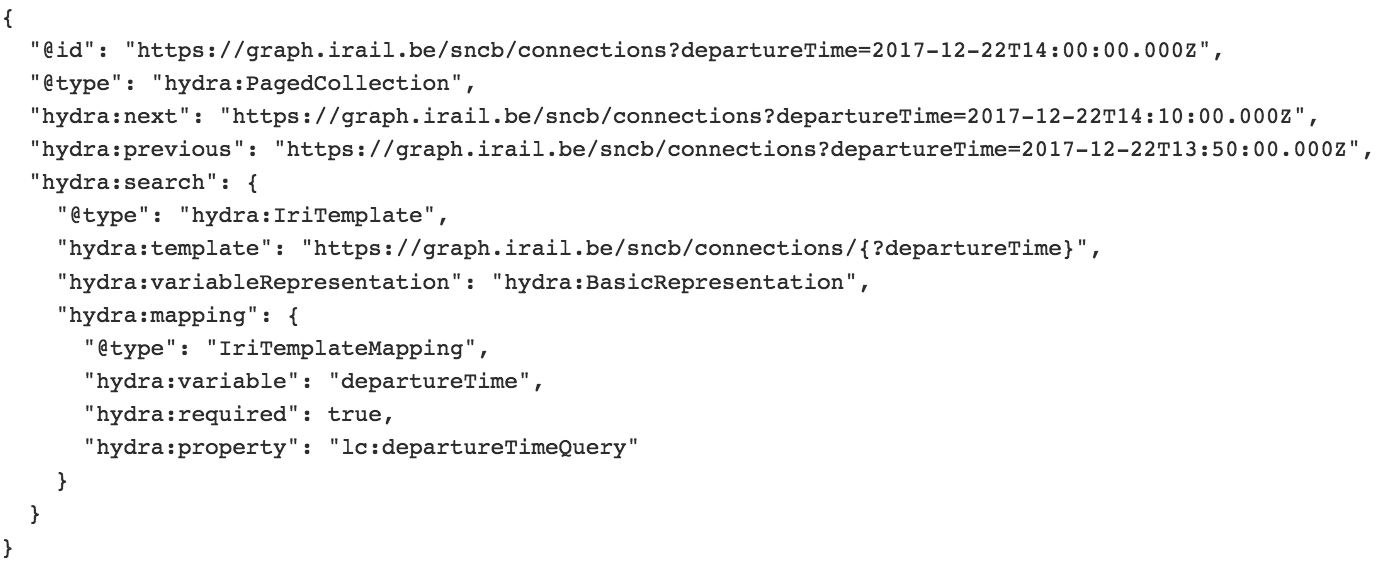
\includegraphics[width=0.5\textwidth]{images/search.png}
	\caption{Metadata LC response}\label{fig:metadata}
\end{figure}

Finally, for each document that is published by a Linked Connections server, a Cross Origin Resource Sharing\footnote{\url{http://enable-cors.org/}} HTTP header must set the property Access-Control-Allow-Origin for sharing the response with any origin. The server also should implement thorough caching strategies, as the cachability is one of the biggest advantages of the Linked Connections framework. Both conditional requests\footnote{\url{https://developer.mozilla.org/en-US/docs/Web/HTTP/Conditional_requests}} as regular caching\footnote{\url{https://developer.mozilla.org/en-US/docs/Web/HTTP/Caching}} are recommended. As every connection will need to have a unique an persistent identifier, an HTTP URI, the server must support at least one RDF1.1 format, such as JSON-LD\cite{world2014json}, TriG\cite{bizer2014rdf} or N-Quads\cite{cyganiak2008n}. The connection URI should follow the Linked Data principles\cite{bizer2009linked}.

\subsection{Real-time in Linked Connections}
%https://github.com/linkedconnections/gtfsrt2lc
As we aforementioned, the transport domain should involve in their route planning algorithms the real-time to provide consistent information to the passengers and improve the current  informational services.  The \textit{de-facto} standard for exchange transport data on the Web, GTFS, has created a version for real-time updates, GTFS-RT.  
Providing globally unique identifiers to the different entities that comprise a public transport network is fundamental to lower the adoption cost of public transport data in route-planning applications. Specifically in the case of live updates about the schedules is important to maintain stable identifiers that remain valid over time. Here we use the Linked Data principles to transform schedule updates given in the GTFS-RT format to Linked Connections and we give the option to serialize them in JSON, CSV or RDF (turtle, N-Triples or JSON-LD) format.

The URI strategy to be used during the conversion process is given following the RFC 6570\footnote{\url{https://tools.ietf.org/html/rfc6570}} specification for URI templates. The parameters used to build the URIs are given following an object-like notation (object.variable) where the left side references a CSV file present in the provided GTFS data source and the right side references a specific column of such file. We use the data from a reference GTFS data source to create the URIs as with only the data present in a GTFS-RT update may not be feasible to create persistent URIs. The GFTS files that can be used to create the URIs are routes and trips files. A simple example is shown in Figure \ref{fig:connection_rt} and an standard template is also available\footnote{\url{https://github.com/linkedconnections/gtfsrt2lc/blob/master/uris_template_example.json}}. As for the variables, any column that exists in those files can be referenced. Next we describe how are the entities URIs build based on these templates :

\begin{itemize}
\item \textbf{stop}: A Linked Connection references two different stops (departure and arrival stop). The data used to build these specific URIs comes directly from the GTFS-RT update, so we do not specify any CSV file and header from the reference GTFS data source. The variable name chosen in our case is the stop\_id but it can be freely named.
\item \textbf{route}: For the route identifier we rely on the routes.route\_short\_name and the trips.trip\_short\_name variables.
\item \textbf{connection}:  For a connection identifier we resort to its departure stop with connection.departureStop, its departure time with connection.departureTime(YYYYMMDD), and the routes.route\_short\_name and the trips.trip\_short\_name. In this case we reference a special entity we called connection which contains the related basic data that can be extracted from a GTFS-RT update for every Linked Connection. A connection entity contains these parameters that can be used on the URIs definition: connection.departureStop, connection.arrivalStop, connection.departureTime and connection.arrivalTime. As both departureTime and arrivalTime are date objects, the expected format can be defined using brackets.
\item \textbf{trip}: In the case of the trip we add the associated connection.departureTime(YYYYMMDD) on top of the route URI.
\end{itemize}

\begin{figure}[t]
	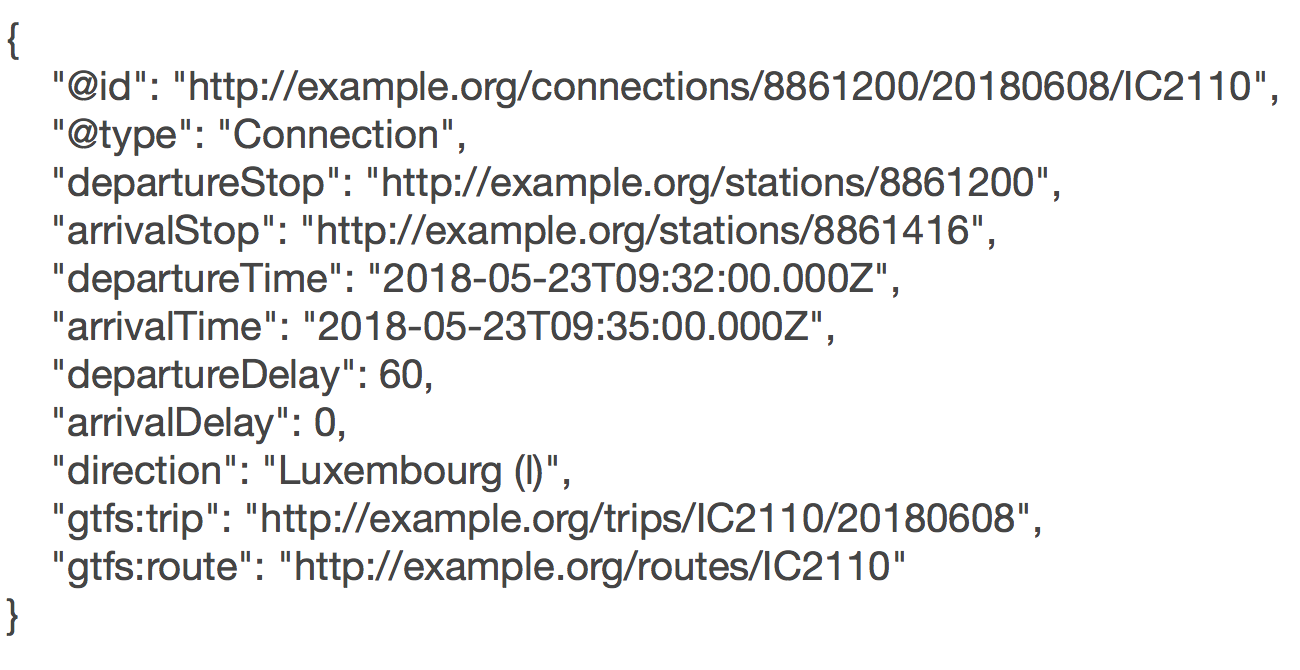
\includegraphics[width=0.47\textwidth]{images/example_connection_rt.png}
	\caption{Real-time connection example}\label{fig:connection_rt}
\end{figure}

Finally, we developed a library\footnote{\url{https://github.com/linkedconnections/gtfsrt2lc}} that analyses the information from an static GTFS dataset and the updates from a GTFS-RT feed, exploits the implicit relations among the CSV files and creates the real-time Linked Connections feed in the desirable format with the help of the URIs template, as it is shown in Figure \ref{fig:gtfsrt2lc}.
\begin{figure}[t]
	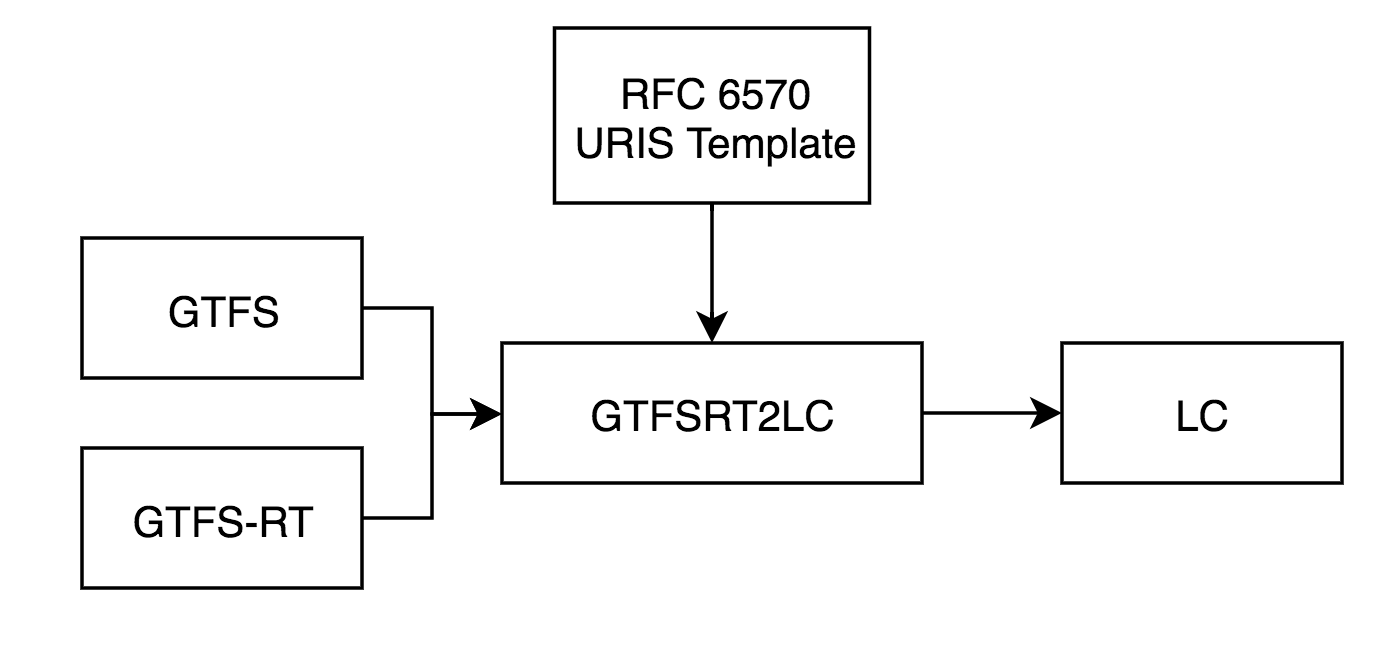
\includegraphics[width=0.47\textwidth]{images/gtfsrt2lc.png}
	\caption{The GTFSRT2LC library}\label{fig:gtfsrt2lc}
\end{figure}


\subsection{Managing real-time and historical with the Linked Connections server}



\subsection{Route planning algorithms}

\section{Evaluation Design}
%data analysis (size, rt or not, etc), implementations used (all), 
\subsection{A running example: Providing reliable access to SNCB}

\section{Results}

\section{Discussion}

\section{Conclusions and Future work}

\begin{acks}
	
\end{acks}

%\begin{figure}[t]
%\includegraphics{}
%\caption{Figure caption.}\label{f1}
%\end{figure}

%\begin{table*}
%\caption{} \label{t1}
%\begin{tabular}{lll}
%\hline
%&&\\
%&&\\
%\hline
%\end{tabular}
%\end{table*}

%%%%%%%%%%% The bibliography starts:

%%%%%%%%%%%%%%%%%%%%%%%%%%%%%%%%%%%%%%%%%%%%%%%%%%%%%%%%%%%%%
%%                  The Bibliography                       %%
%%                                                         %%
%%  ios1.bst will be used to                               %%
%%  create a .BBL file for submission.                     %%
%%                                                         %%
%%                                                         %%
%%  Note that the displayed Bibliography will not          %%
%%  necessarily be rendered by Latex exactly as specified  %%
%%  in the online Instructions for Authors.                %%
%%                                                         %%
%%%%%%%%%%%%%%%%%%%%%%%%%%%%%%%%%%%%%%%%%%%%%%%%%%%%%%%%%%%%%


\nocite{*}
% if your bibliography is in bibtex format, use those commands:
\bibliographystyle{ios1}           % Style BST file.
\bibliography{bibliography}        % Bibliography file (usually '*.bib')

% or include bibliography directly:
%\begin{thebibliography}{0}
%\bibitem{r1} F. Author, Information about cited object.
%
%\bibitem{r2} S. Author and T. Author, Information about cited object.
%\end{thebibliography}

\end{document}
